\documentclass[graphics]{beamer}
\usepackage{graphicx}
\usepackage{listings} % Syntax highlighing
\usepackage{fancyvrb} % Inline verbatim
\usepackage{hyperref} % Hyperlinks
\hypersetup{pdfpagemode=FullScreen}

\usetheme{Boadilla}
\title{Lecture 2: Architecture \& Number Systems}
\author{UMBC CMSC 104}
\date{L2}

\begin{document}

\begin{frame}{}
\centering
    Machine Architecture and Number Systems
\end{frame}

\begin{frame}{Why are we in this course?}
    \center{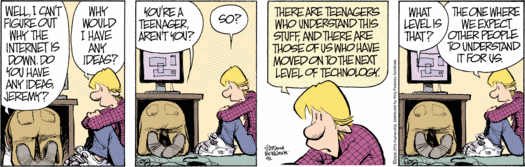
\includegraphics[scale=0.61]{L02_ArchNumbersSystems/L2_p2.png}}
    
    \newline
    Remember: ``There are no stupid questions, just stupid people who don't know they should be asking something''
\end{frame}

\begin{frame}{Machine Architecture \& Number Systems}
Topics:
\begin{itemize}
    \item Major computer components
    \item Bits, bytes, words
    \item The Decimal number system
    \item The Binary number system
    \item Converting from Binary to Decimal
    \item Converting from Decimal to Binary
    \item The Hexadecimal number system
\end{itemize}
    
\end{frame}

\begin{frame}{Some People Think a Computer is...}
    \centering
    \only<1>{
        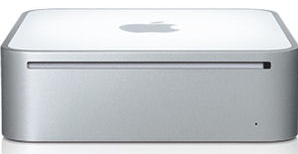
\includegraphics[scale=0.8]{L02_ArchNumbersSystems/L2_p4.png}
    }
    \only<2>{
        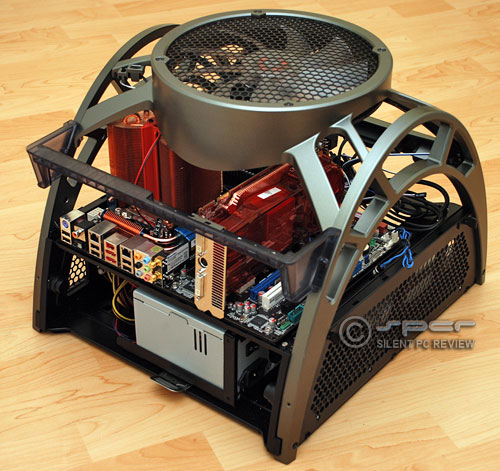
\includegraphics[scale=0.65]{L02_ArchNumbersSystems/L2_p5.png}
    }
\end{frame}

\begin{frame}{Major Computer Components}
    \begin{itemize}
        \item Central Processing Unit (CPU)
        \item Bus
        \item Main memory (RAM)
        \item Secondary storage media
        \item Input/Output (I/O) devices
    \end{itemize}
\end{frame}

\begin{frame}{Schematic Diagram of a Computer}
    \centering
    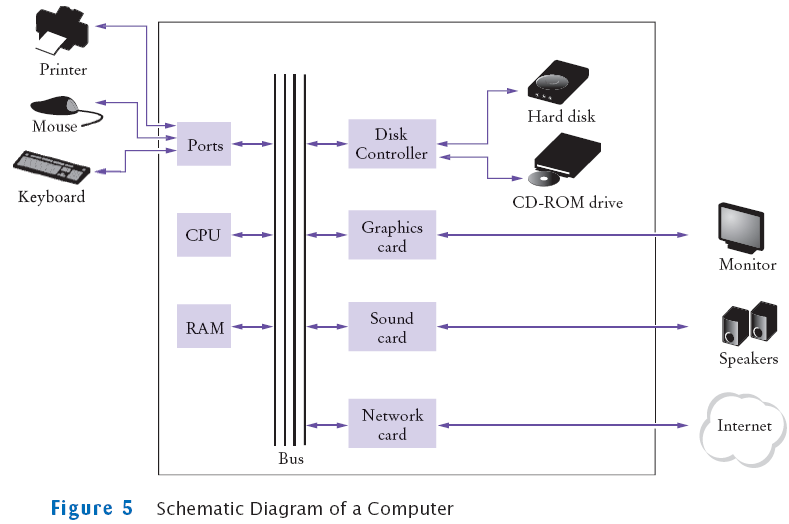
\includegraphics[scale=0.6]{L02_ArchNumbersSystems/L2_p7.png}
    \footnotesize{Diagram taken from Java Concepts, Fourth Edition}
\end{frame}

\begin{frame}{Realistic Diagram of Computer Components}
\centering
    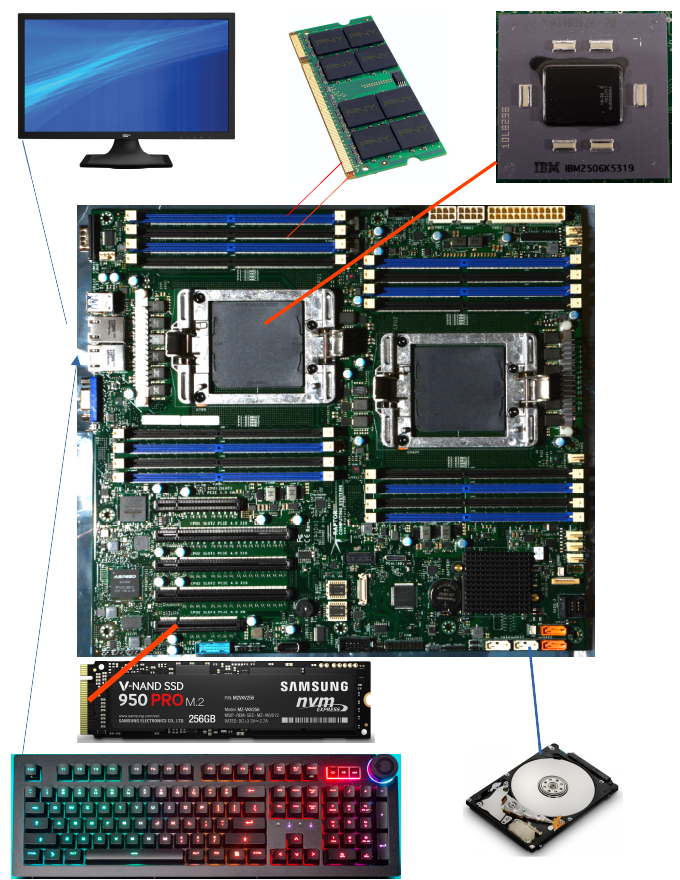
\includegraphics[scale=0.25]{L02_ArchNumbersSystems/L2_p8.png}
\end{frame}

\begin{frame}{The CPU}
\begin{columns}
    \column{0.6\textwidth}
    \begin{itemize}
        \item Central Processing Unit
        \item The ``brain'' of the computer
        \item Controls all other computer functions
        \item Sometimes called a microprocessor or simply processor
        \item There are different processors for different types of devices (the processor in your computer is very different compared to the processor in your phone)
    \end{itemize}
     \column{0.4\textwidth}
    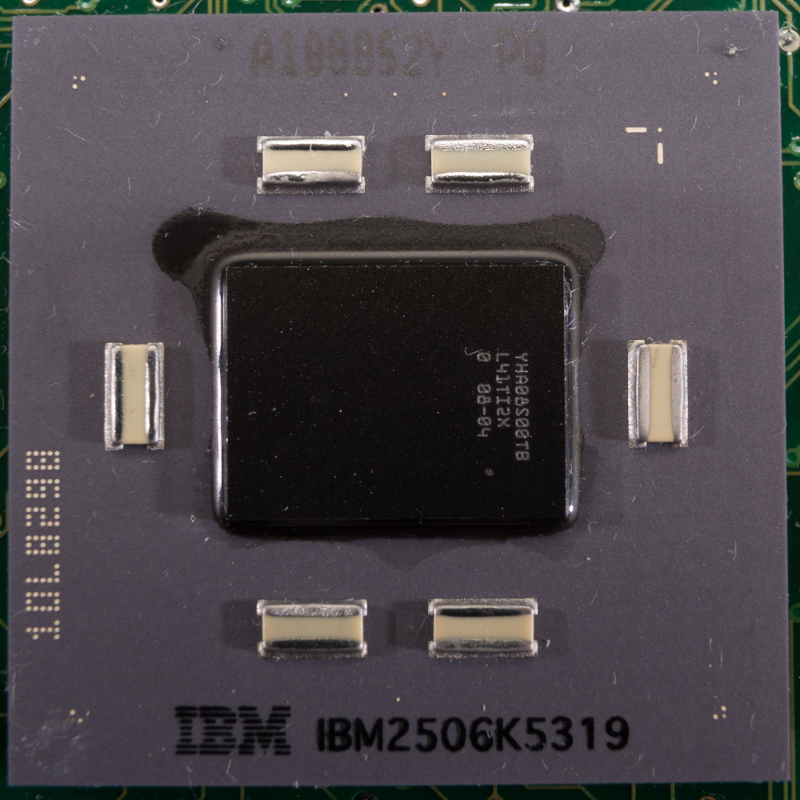
\includegraphics[scale=0.6]{L02_ArchNumbersSystems/L2_p8_cpu.png}
    \end{columns}
\end{frame}

\begin{frame}{The Bus}
    \begin{itemize}
        \item Computer components are connected by a bus
        \item A bus is a group of parallel wires which carry control signals \& data between components.
        \item USB = Universal Serial \underline{Bus}
    \end{itemize}
\end{frame}

\begin{frame}{Main Memory}
\only<1>{
    \begin{columns}
        \column{0.6\textwidth}
        \begin{itemize}
            \item Main memory holds information needed to run the computer, which includes information about the operating system, programs which are running, and everything else which makes the computer usable.
        \end{itemize}
    \column{0.4\textwidth}
        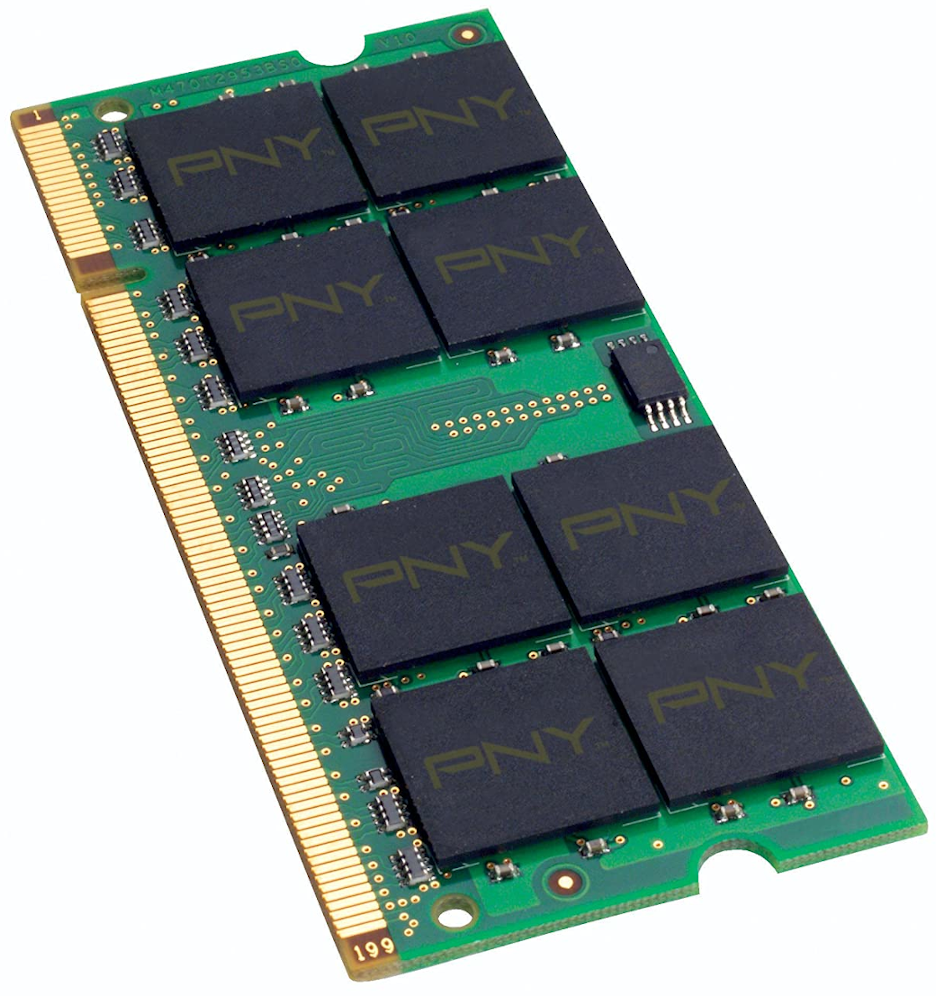
\includegraphics[scale=0.5]{L02_ArchNumbersSystems/L2_p8_ram.png}
    \end{columns}
    }
\only<2> {
    \begin{itemize}
        \item Main memory is made up of transistors.
        \item If the transistor is closed, then it's state is said to be 1, or ON.
        \item If the transistor is open, then it's state is said to be 0, or OFF.
        \item Keeping track of off and on states is why computers use binary numbers.
    \end{itemize}
}
\only<3> {
    \begin{itemize}
        \item Every eight bits is known as a \textit{byte}.
        \item Each of these bytes as uniquely numbered, which is it's \textit{address}.
        \item Memory is volatile storage, meaning that the information is lost when the computer no longer has electricity.
    \end{itemize}
}
\only<4> {
    \begin{itemize}
        \item Other computer components can:
        \begin{itemize}
            \item get the information held at a particular address in memory, known as a \textit{READ},
            \item and store information at a particular address in memory, known as a \textit{WRITE}.
        \end{itemize}
        \item Writing to a memory location alters it's contents, the prior information is lost.
        \item Reading from a memory location does not alter its contents.
        \item Example: when browsing the Internet, the browser sends information to another website.
        \begin{itemize}
            \item The browser writes information to memory
            \item The network card reads the information, sends data across the network
            \item The network card gets information from the server, writes data to memory
            \item The web browser reads the memory and displays it to you.
        \end{itemize}
    \end{itemize}
}
\only<5> {
    \begin{itemize}
        \item All addresses in memory can be accessed in the same amount of time.
        \item The computer doesn't start at address 0 and read until we get to the address we really want (\textit{sequential access}).
        \item The computer goes directly to the address we want and accesses the data (known as \textit{direct} or \textit{random access}).
        \item This is where RAM gets it's name: \textit{Random Access Memory}.
    \end{itemize}
}
\only<6> {
    \begin{itemize}
        \item ``Stupid question'': Why does adding more RAM make the computer faster, or seem faster?
        \item Answer: This is a complicated situation, it has to do with swapping/paging, and multiprocessing.
        \item Portions of memory which aren't used often are saved to the hard drive, to free up memory for programs which are currently running, known as \textit{swapping}. More RAM means more information can be stored at once, and RAM is always faster than the hard drive.
    \end{itemize}
}
\end{frame}

\begin{frame}{Secondary Storage}
    \begin{itemize}
        \item From faster to slower:
        \begin{itemize}
            \item Hard drives (random access)
            \item USB thumb drives (random access)
            \item Optical: CD, DVD, Blu-ray drives (random access)
            \item Floppy drives (random access)
            \item Tapes (sequential access)
        \end{itemize}
        \item These types are known as persistent or permanent storage, since they're non-volatile.
    \end{itemize}
    \begin{columns}
        \column{0.4\textwidth}
            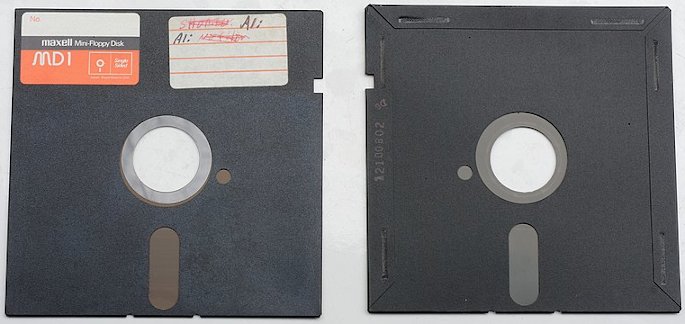
\includegraphics[scale=0.20]{L02_ArchNumbersSystems/L2_p17_525.png}
        \column{0.6\textwidth}
            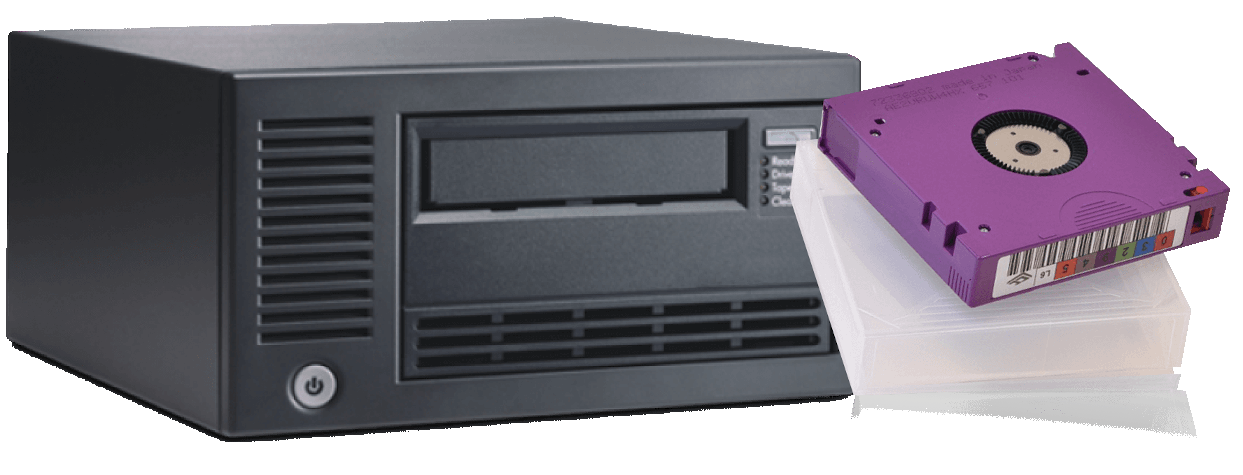
\includegraphics[scale=0.17]{L02_ArchNumbersSystems/L2_p17_tape.png}
    \end{columns}
\end{frame}

\begin{frame}{Input/Output (I/O) Devices}
    \begin{itemize}
        \item Information input and output is handed by I/O devices, also known as peripheral devices
        \item Examples:
        \begin{itemize}
            \item Monitor (output)
            \item Keyboard (input)
            \item Mouse (input)
            \item Joystick, gamepad (input)
            \item Disk drive (input \& output)
            \item CD-ROM, DVD-ROM (input)
            \item CD, DVD burner (input \& output)
            \item Printer (output)
            \item Scanner (input)
            \item Network card (input \& output)
            \item Sound card (input \& output)
        \end{itemize}
    \end{itemize}
\end{frame}

\begin{frame}{Opening MS Word}
    \begin{itemize}
        \item Use the mouse to select MS Word
        \item The CPU requests the MS Word application
        \item MS Word is loaded from the hard drive to main memory
        \item The CPU reads instructions from main memory and executes them one at a time
        \item MS Word appears on your monitor
    \end{itemize}
\end{frame}

\begin{frame}{Bits, Bytes, Words}
    \begin{itemize}
        \item A bit is a single binary digit (zero or one)
        \item A byte is 8 bits
        \item A word is 32 bits, or 4 bytes
        \item Long word = 8 bytes = 64 bits
        \item Quad word = 16 bytes = 128 bits
        \item Programming languages use these standard number of bits when organizing data
    \end{itemize}
\end{frame}

\begin{frame}{Number Systems}
    
\end{frame}

\end{document}